\documentclass[a4paper, 12pt]{article}%тип документа

%отступы
\usepackage[left=0.6cm,right=1cm,top=2cm,bottom=3cm,bindingoffset=0cm]{geometry}
\setlength{\parindent}{5ex}

%Русский язык
\usepackage[T2A]{fontenc} %кодировка
\usepackage[utf8]{inputenc} %кодировка исходного кода
\usepackage[english,russian]{babel} %локализация и переносы

%Вставка картинок
\usepackage{graphicx}
\graphicspath{{pictures/}}
\DeclareGraphicsExtensions{.pdf,.png,.jpg}

%Графики
\usepackage{pgfplots}
\pgfplotsset{compat=1.9}

%Математика
\usepackage{amsmath, amsfonts, amssymb, amsthm, mathtools}

%Таблицы
\usepackage{longtable} 
\usepackage{float}

%Римские цифры
\newcommand{\RomanNumeralCaps}[1]{\uppercase\expandafter{\romannumeral#1}}

\usepackage{multirow}


\begin{document}
	\begin{titlepage}
		\begin{center}
			\textsc{Федеральное государственное автономное образовательное учреждение высшего образования«Московский физико-технический институт (национальный исследовательский университет)»\\[5mm]
			}
			
			\vfill
			
			\textbf{Отчёт по лабораторной работы 4.3.4 \\[3mm]
				ПРЕОБРАЗОВАНИЕ ФУРЬЕ В ОПТИКЕ
				\\[50mm]
			}
			
		\end{center}
		
		\hfill
		\begin{minipage}{.5\textwidth}
			Выполнил студент:\\[2mm]
			Сериков Алексей Романович\\[2mm]
			группа: Б03-103\\[5mm]
			
		\end{minipage}
		\vfill
		\begin{center}
			Москва, 2023 г.
		\end{center}
		
	\end{titlepage}
	
	\newpage
	\textbf{Аннотация}\\
	
	
	\textbf{Цель работы: }\\
	
	Определить размеры щели, определить периоды сеток; исследовать изображение щели.
	
	
	\textbf{В работе используются: }\\
	
	Гелий-неоновый лазер, кассета с набором сеток разного периода, щель с микрометрическим винтом, линзы, экран, линейка.
	
	
		\textbf{Теория:}
	
	Рассмотрим дифракцию плоской монохроматической волны на синусоидальной амплитудной решётке. Пусть решётка с периодом d расположена в $t = 0$, а её штрихи ориентированы вдоль $OY$. Тогда функция пропускания:
	\[
	t(x) = \beta  + \alpha cos(ux) = \beta + \alpha \frac{e^{iux} + e^{-iux}}{2},
	\]
	где $\alpha, \beta = const, u = \frac{2 \pi}{d}$.
	
	Если на решётку падает плоская моно волна вдоль $OZ$:
	\[
	E(\vec r, t) = E_0 e^{-i(\omega t - kz)},
	\]
	то на выходе получим три плоских волны:
	\[
	E_1 = \beta E_0 e^{-i (\omega t - kz)};
	\]
	\[
	E_2 = \frac{\alpha}{2} E_0 e^{-i (\omega t - ux - \sqrt{k^2 - u^2}z)};
	\]
	\[
	E_3 = \frac{\alpha}{2} E_0 e^{-i (\omega t + ux - \sqrt{k^2 - u^2}z)},
	\]
	где $\omega$ "--- круговая частота, $k = \frac{2 \pi}{\lambda}$ "--- волновой вектор, $E_0$ "--- амплитуда.
	Каждая из этих трёх волн фокусируется линзой в точку в задней фокальной плоскости. Волна $E_1$ (вдоль $OZ$) фокусируется в начало координат, волны $E_2$ И $E_3$ (распространяются в направлении $\sin \theta = \pm \frac{u}{k}$) фокусируются в точке $x_1 = \pm \frac{Fu}{k} = \pm {F \lambda}{d}$, где $F$ "--- фокусное расстояние линзы.
	
	Теорема Фурье в комплексной форме:
	\[
	t(x) = \sum_{n = - \infty}^\infty C_n e^{inux},
	\]
	сумма бесконечного множества канонических составляющих, имеющие кратные частоты.
	Картина, наблюдаемая в фурье-плоскости, представляет собой эквидистантный набор точек с координатами и амплитудами, пропорциональными $C_n$:
	\[
	x_n = \frac{Fu}{k} = \frac{F \lambda}{d}n.
	\]
	При освещении транспаранта плоской моно волной картина, наблюдаемая в задней фокальной плоскости линзы, установленной за транспарантом, представляет собой фурье-образ функции пропускания транспаранта.
	Для того, чтобы найти фурье-образ функции пропускания, достаточно определить только пространственные частоты и соотношение между амплитудами плоских волн на выходе. Для амплитудной синусоидальной решётки получаем три плоских волны с частотами $0, +u, -u$ и амплитудами, пропорциональными $\beta, \frac{\alpha}{2}, \frac{\alpha}{2}$.
	\begin{figure}[H]
		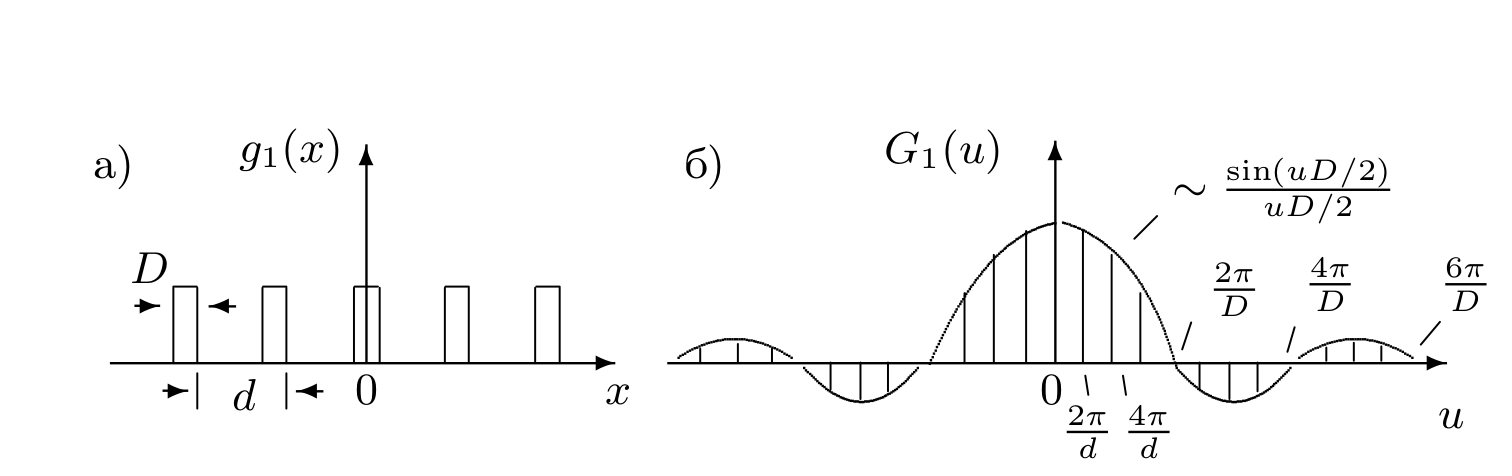
\includegraphics[width = 0.6\linewidth]{5.png}
		\caption*{а) функция пропускания дифракционной решётки (последовательности прозрачных и непрозрачных полос);
			
			б) $G_1 (u)$ "--- спектр функции пропускания дифракционной решётки}
	\end{figure}	
	Пространственное преобразование Фурье может осуществляться и в свободном пространстве при наблюдении дифракции Фраунгофера.
	Если размеры дифракционной решётки неограничены, то дифракционные максимумы бесконечно узки. Чем меньше размер решётки (полное число щелей), тем шире каждый отдельный максимум.
	
	Направление на главные максимумы $\theta_n = \frac{u n}{k} = \frac{\lambda n}{d}$ ($N$ "--- целое число) определяется периодом решётки d, а распределение амплитуд в спектре "--- фурье-образом функции пропускания отдельного штриха:
	\[
	g_2 (x) = \begin{cases} 1, & - \frac{D}{2} \leq x \leq \frac{D}{2} \\
		0, & - \frac{D}{2} > x > \frac{D}{2}
	\end{cases}
	\]
	Вследствие периодичности $g_2(x)$, её фурье-образ представляется непрерывным множеством точек и определяется интегральным преобразованием Фурье:
	\[
	g(x) = \frac{1}{2 \pi} \int_{-\infty}^{+\infty} G(u) e^{iux} du,
	\]
	\[
	G(u) = \int_{-\infty}^{+\infty} g(x) e^{-iux}dx.
	\]
	В таком виде $g(x)$ и $G(u)$ представляют собой пару преобразований Фурье: $G(u)$ "--- спектр или фурье-образ функции $g(x)$.
	\[
	G_2 (u) = \int_{-\infty}^{+\infty} g_2 (x) e^{-iux} dx  = \int_{-D/2}^{+D/2} e^{-iux} dx = D \frac{\sin \frac{uD}{2}}{\frac{uD}{2}}.
	\]
	Введём понятие протяженности функции пропускания транспаранта ($\Delta x$) и ширины её спектра ($\Delta u$), тогда соотношение неопределённости принимает вид:
	\[
	\Delta x \cdot \Delta u = \frac{2 \pi}{D} \cdot D = 2 \pi.
	\]
	Размер же малого объекта можно рассчитать, увеличив его изображение с помощью линзы.
	
	\textbf{Метод Аббе}
	Рассмотрим схему образования изображения. Пусть предмет расположен от линзы на большем расстоянии, чем фокусное, тогда существует сопряжённая предметной плоскости плоскость, где образуется изображение. Аббе предложил рассматривать схему прохождения в два этапа: сначала рассматривается первичное изображение (спектр в задней фокальной плоскости), затем это изображение рассматривается как источник волн, создающий изображение в другой плоскости (вторичное изображение). Этот подход опирается на принцип Гюйгенса-Френеля, согласно которому любой участок волнового фронта можно рассматривать как источник излучения. Под словами <<линза дважды осуществляет преобразование Фурье>> подразумевается следующее: сначала в задней фокальной плоскости линзы получается световое поле, соответствующее фурье-образу функции пропускания предмета (с точностью до фазы), а затем на промежутке между фокальной плоскостью и плоскостью изображения осуществляется обратное преобразование Фурье, в результате чего восстанавливается изображение предмета.
	
	
\textbf{Ход работы и обработка результатов.}\\

\RomanNumeralCaps 1 \textit{Определение ширины щели с помощью линзы:}\\


	\begin{figure}[H]
		\begin{center}
		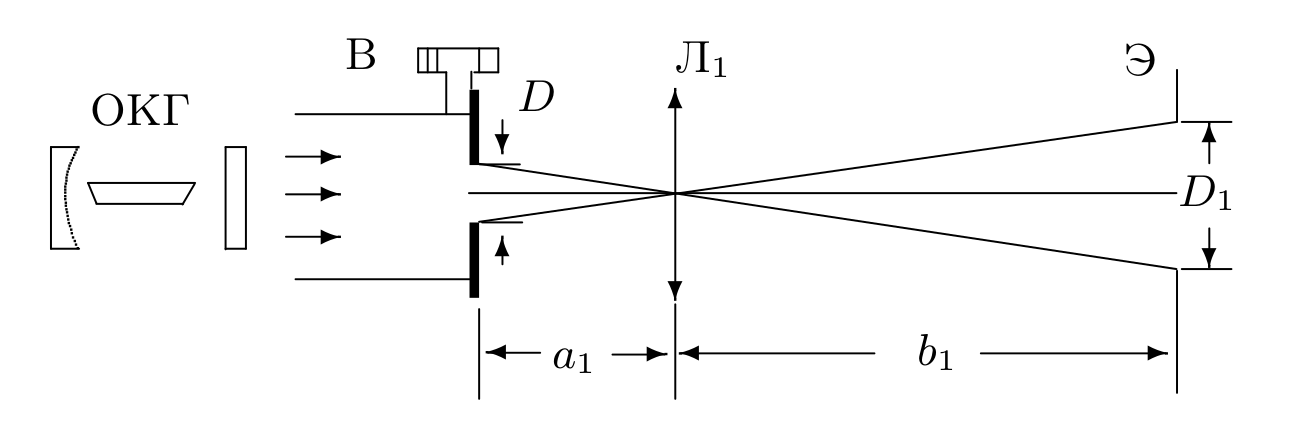
\includegraphics[width = 0.6\linewidth]{1.png}
		\caption{Схема для определения ширины щели с помощью линзы}
		\end{center}
	\end{figure}	
	
	$F_1 = 43$ мм и $D_0 = 100$ мкм.
	
	\begin{table}[H]
		\centering
		\begin{tabular}{|c|c|c|c|c|c|c|c|c|c|c|}  \hline
			$D,$ мкм & 150 & 200 & 250 & 300 & 350 & 400 & 450 & 500 & 550 & 600\\\hline
			$D - D_0, $\ мкм & 50 & 100 & 150 & 200 & 250 & 300 & 350 & 400 & 450 & 500 \\\hline
			$D_1,$ мм & 2 & 2.5 & 3 & 4 & 5 & 6 & 7 & 8 & 9 & 10 \\\hline
			$D_\text{л},$ мкм & 76 & 96 & 115 & 153 & 192 & 230 & 269 & 307 & 346 & 384
			\\\hline
		\end{tabular}
	\end{table}
	\[
	a_1 = 5.0 \pm 0.5, \text{см}; \quad b_1 = 130.0 \pm 0.5, \text{см}; \quad L = 135.0 \pm 0.5, \text{см}.
	\]
	
	\[
	\text{В пределах погрешности} \quad  L = a_1 + b_1. \]
	\[ 
	\text{Г} = \frac{b_1}{a_1} = \frac{130}{5} = 26 \pm 1
	\]
	
	
	\newpage
\RomanNumeralCaps 2 \textit{Определение ширины щели по её спектру:}
	
	\begin{figure}[H]
		\begin{center}
		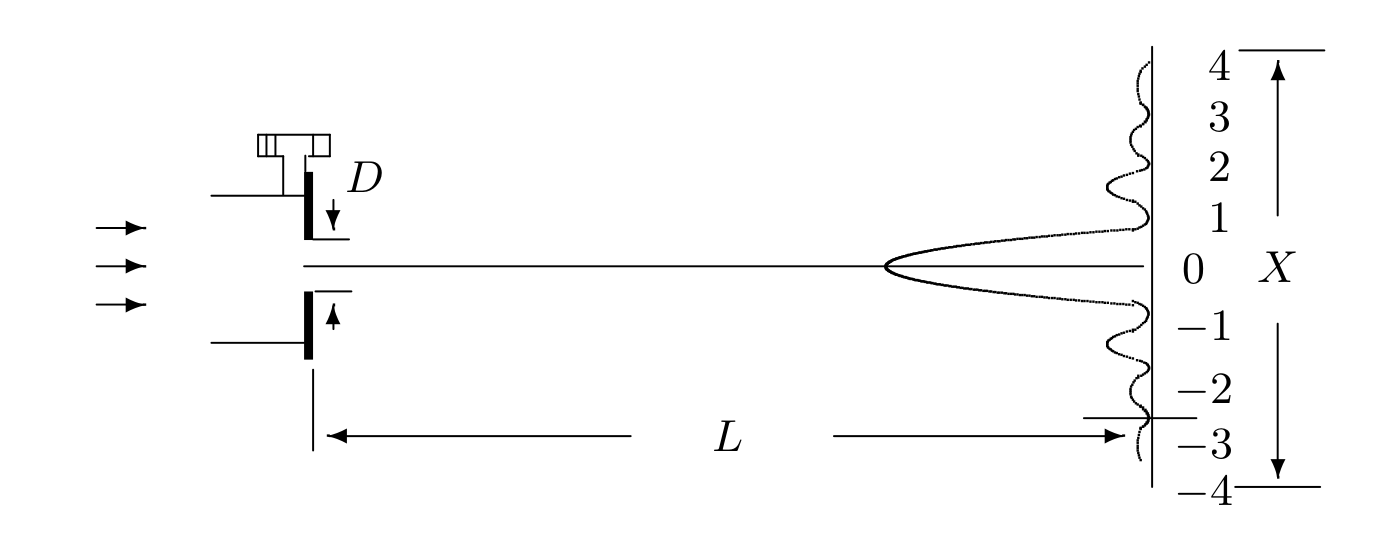
\includegraphics[width = 0.6\linewidth]{2.png}
		\caption*{Схема для определения ширины щели по спектру}
	\end{center}
	\end{figure}
	\begin{table}[H]
		\centering
		\begin{tabular}{|c|c|c|c|c|c|c|}  \hline
			$x(m)$, мм & 180 & 190& 130 & 140 & 160 & 200  \\\hline
			$m$ & 3 & 9 & 10 & 14 & 24 & 37\\\hline
			$\Delta x,$мм & 30.0 & 10.6 & 6.5 & 5.0 & 3.3 & 2.7 \\\hline
			$D_c,$ мкм & 28.4 & 80.8 & 131.3 & 170.6 & 258.5 & 315.9\\\hline
			$D,$ мкм & 150 & 200 & 250 & 300 & 350 & 400\\\hline
			
		\end{tabular}
	\end{table}
	\[
	\Delta x = \frac{x}{2m} = \frac{\lambda}{D_c}L,
	\]	
	где $L = 135.0 \pm 0.5 \text{см}, \lambda = 5320\ \dot A $.
	
	Построим на одном графике зависимости $D_{л} = f(D), D_{c} = f(D)$:
	\begin{figure}[H]
		\begin{center}
			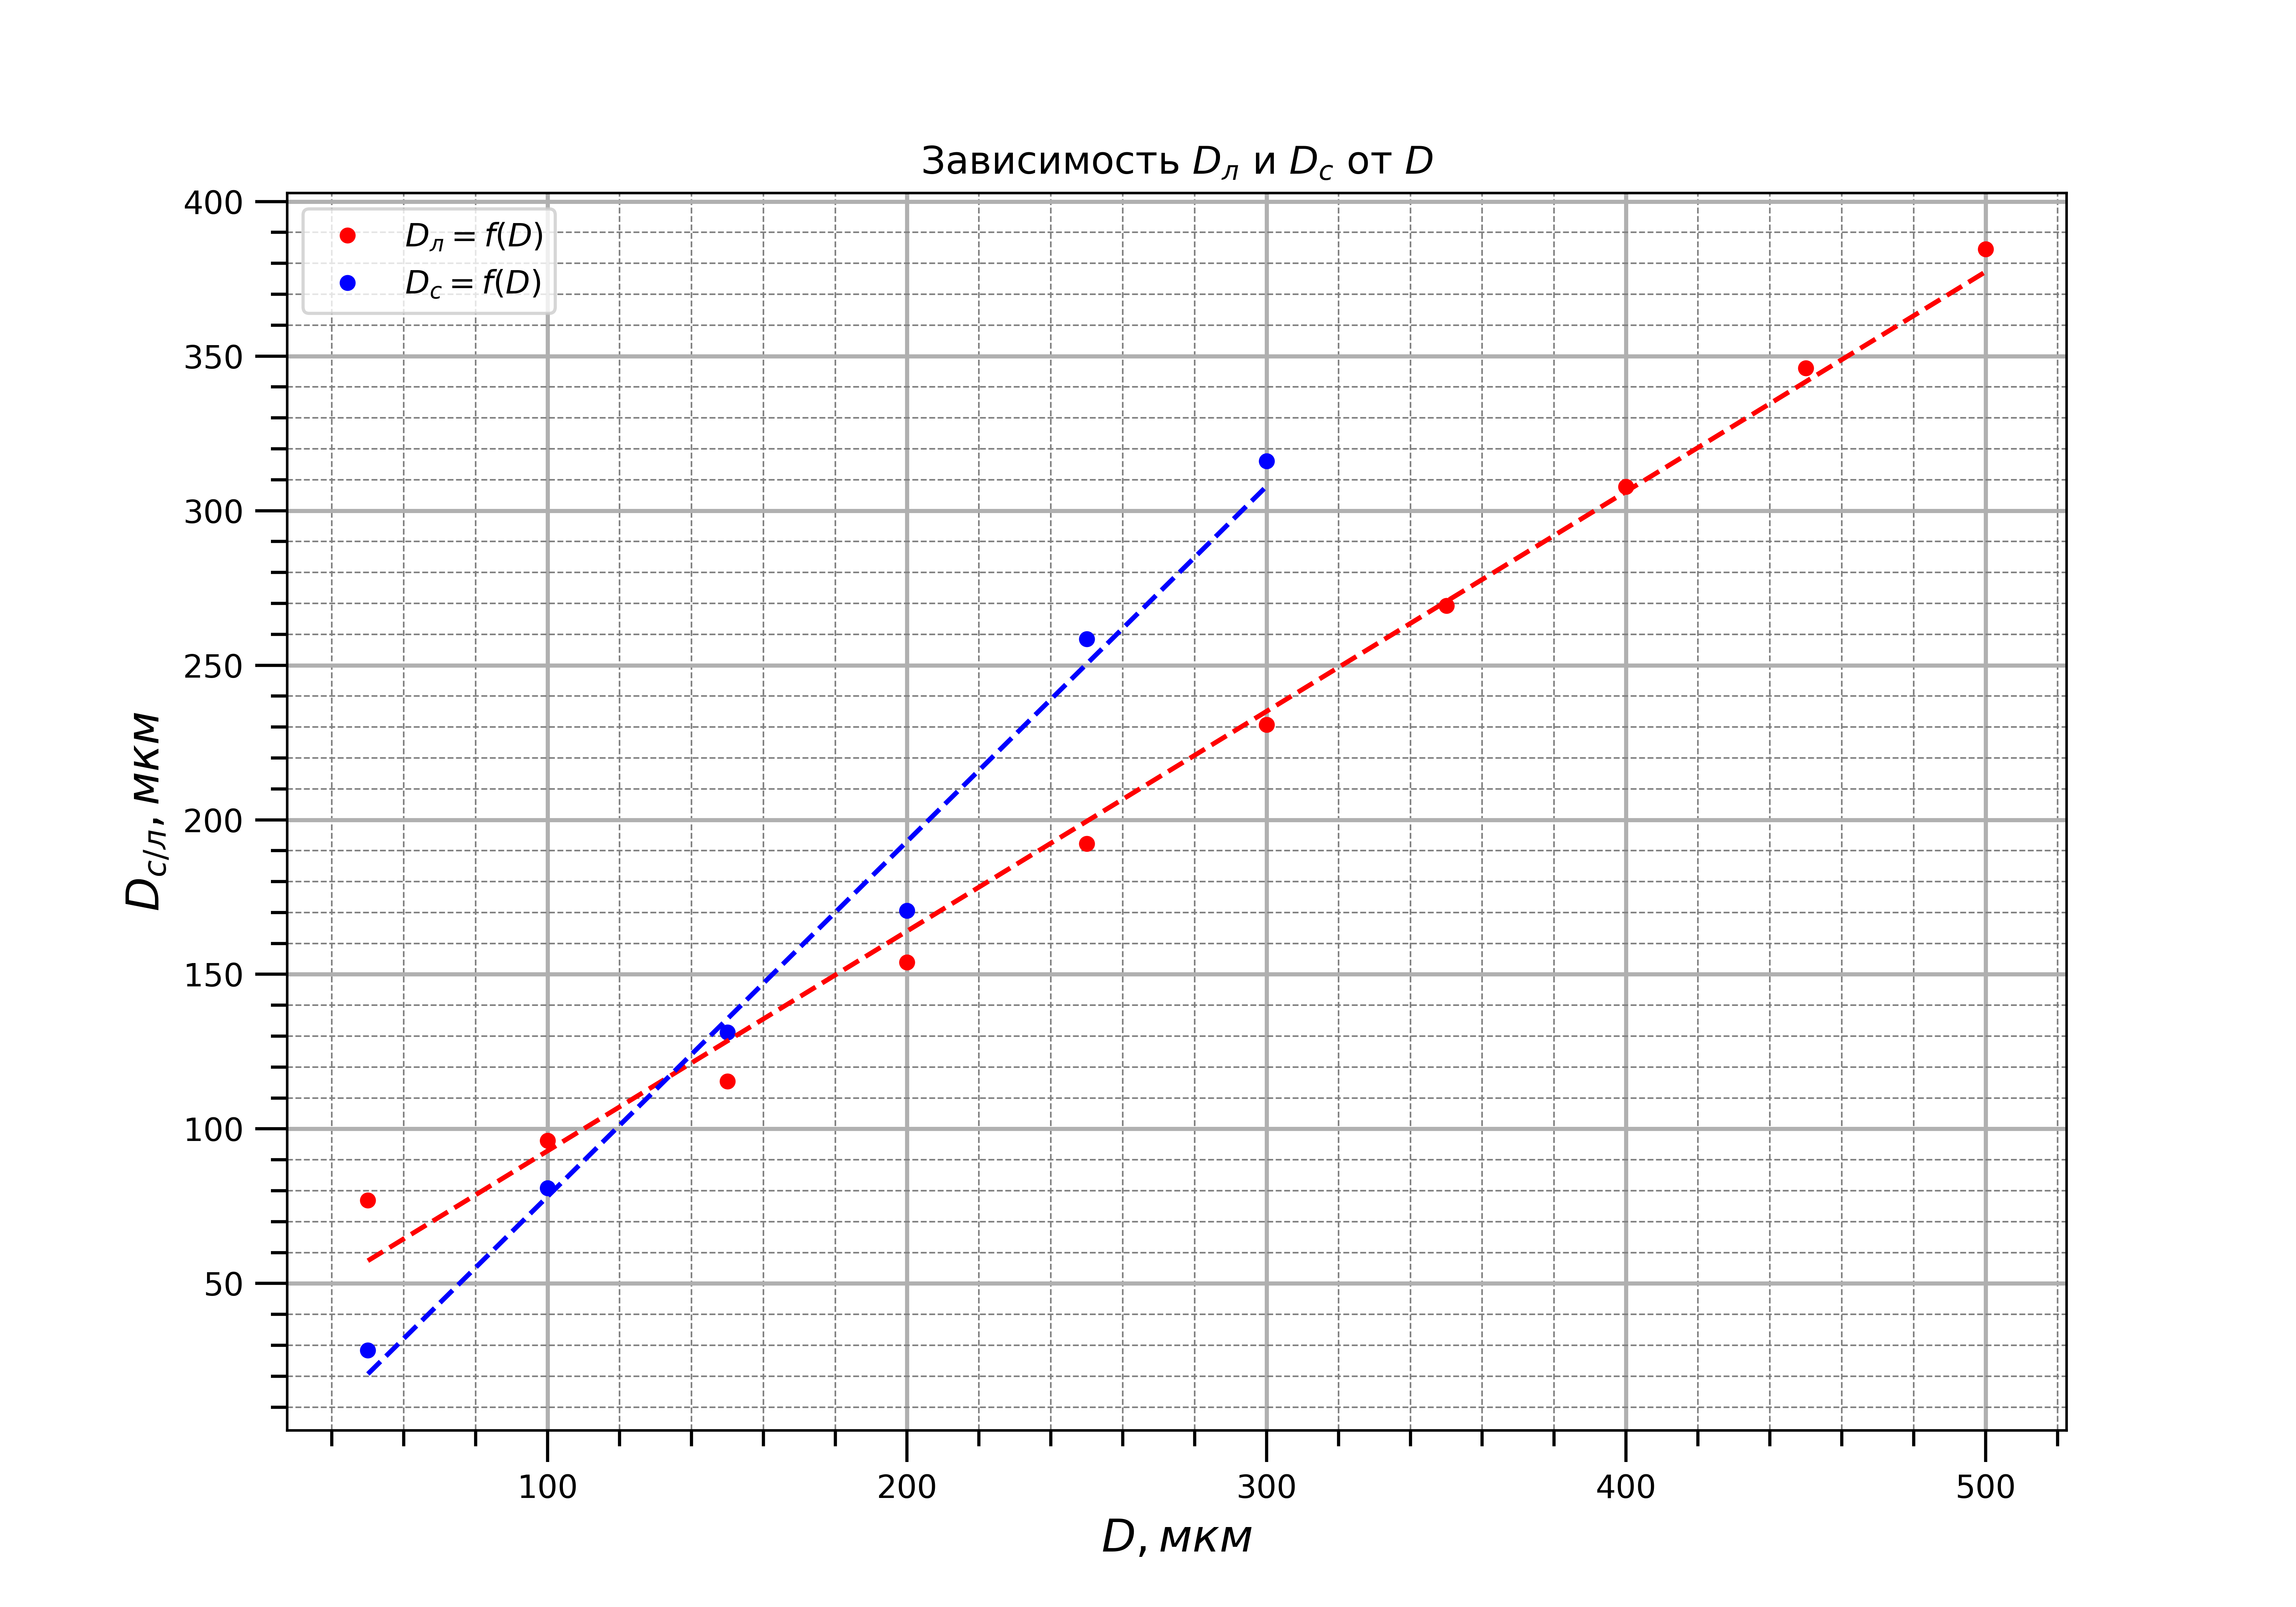
\includegraphics[width=0.6\linewidth]{Dl_Dc.png}
			\caption{График зависимости расчетных данных от прямых измерений}
		\end{center}
	\end{figure}
	
	
	\RomanNumeralCaps 3 \textit{Определение периода решёток по спектру на удалённом экране:}
	Рассчитаем расстояния $\Delta x$ между соседними максимумами и определим период каждой решётки $d_c$, используя соотношения:
	\[
	\Delta x = \frac{x}{2 m} = \frac{\lambda}{d_c} L
	\]
	
	\[
	L = 134 \text{см}
	\]
	\begin{table}[H]
		\centering
		\begin{tabular}{|c|c|c|c|}  \hline
			\textnumero\ решётки & 1 & 2 & 3 \\\hline
			$x(m),$ мм & 87 & 173 & 144 \\\hline
			$m$ & 3 & 3 & 1 \\\hline
			$\Delta x,$ мм & 14.5 & 57.6 & 144 \\\hline
			$d_c,$ мкм & 58.5 & 14.7 & 8.6  \\\hline
		\end{tabular}
	\end{table}



\RomanNumeralCaps 4 \textit{Определение периода решёток по увеличенному изображению спектра:}
	
	\begin{figure}[H]
		\begin{center}
		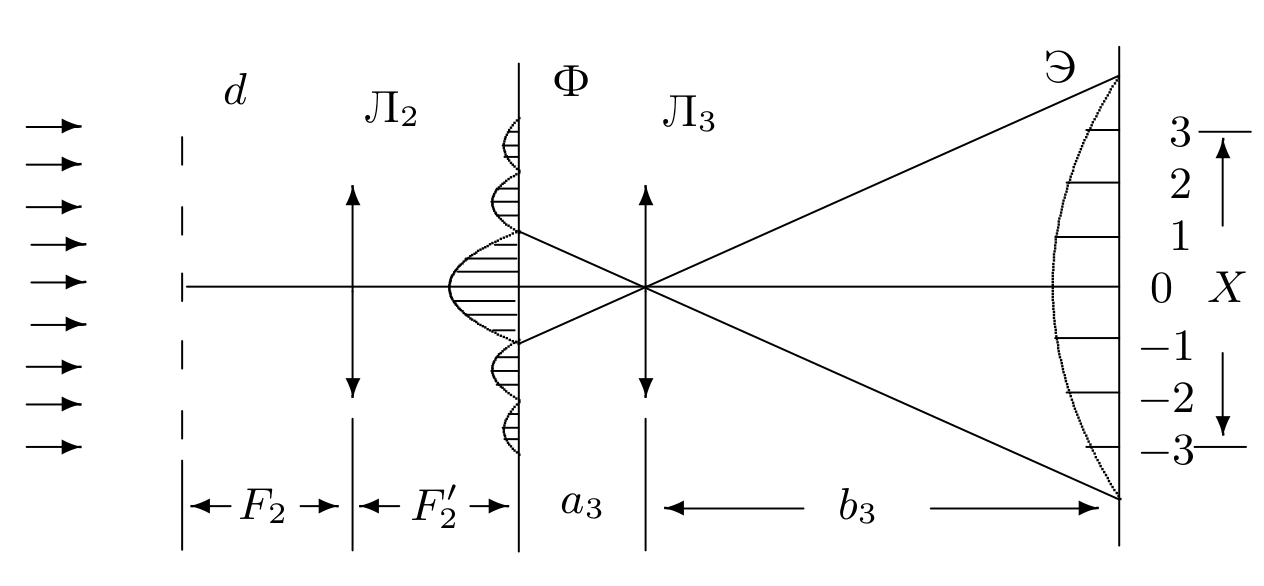
\includegraphics[width = 0.6\linewidth]{3.png}
		\caption{Схема определения периода решётки по увеличенному изображению спектра}
		\end{center}
	\end{figure}
	Установим линзу 2 на расстоянии $F_2$ от кассеты. Так как $b_3 \gg a_3$, то $a_3 \approx F_3$ и расстояние между линзами $= F_2 + F_3$. 
	\[
	F_2 = 110\text{мм}; \quad F_3 = 43 \text{мм}; \quad a_3 = 45 \pm 0.1 \text{мм}; \quad b_3 = 107 \pm 1\ \text{см};
	\]
	
	\[
	\text{Г}_3 = \frac{b_3}{a_3} = \frac{107}{4.5} = 23.7 \pm 1.6
	\]
	Измерим $x$ и $m$ для всех сеток, где это возможно. Зная увеличение линзы, рассчитаем расстояние между максимумами $\Delta x$ плоскости Ф, а затем период сетки $d_c$:
	\[
	\Delta x = \frac{x}{\text{Г}_3} = \frac{\lambda}{d_c} F_2
	\]
	\begin{table}[H]
		\centering
		\begin{tabular}{|c|c|c|c|}  \hline
			\textnumero\ решётки & 1 & 2 & 3  \\\hline
			$x(m),\ мм$ & - & 100 & 152  \\\hline
			$m$ & - & 1 & 3  \\\hline
			$\Delta x,\ мм$ & - & 4.2 & 6.4  \\\hline
			$d_c,\ мкм$  & - & 23.0 & 15.1  \\\hline
		\end{tabular}
	\end{table}

\newpage

\RomanNumeralCaps 5 \textit{Мультиплицирование}
	\begin{figure}[H]
		\begin{center}
		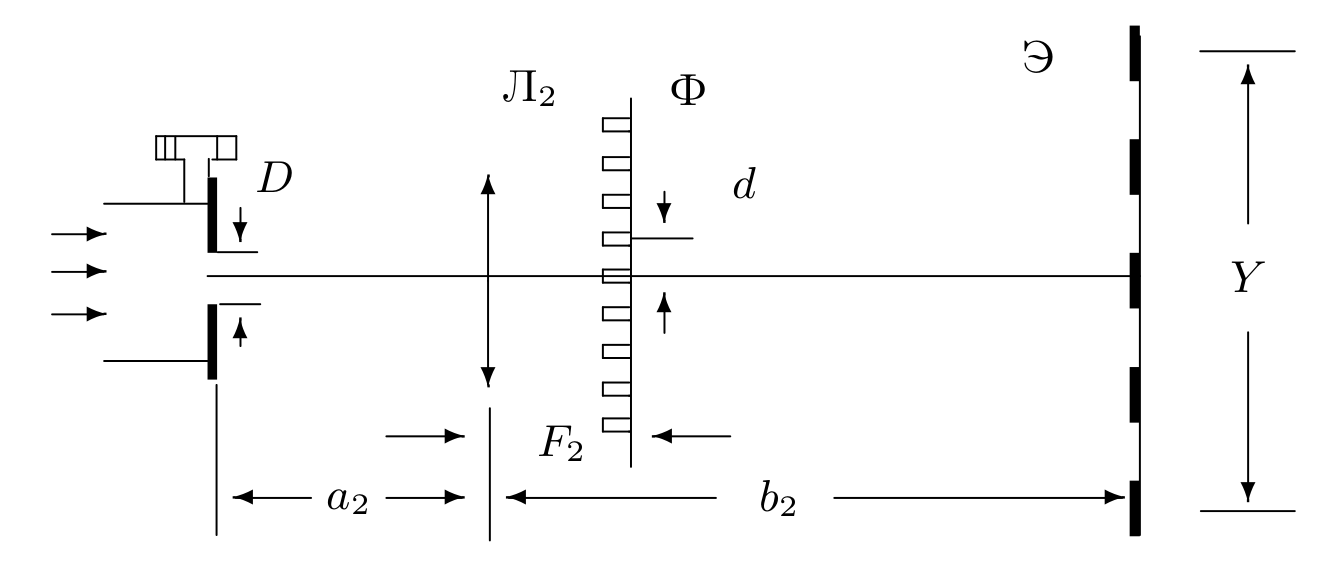
\includegraphics[width = 0.6\linewidth]{4.png}
		\caption{Схема для наблюдения мультиплицирования}
		\end{center}
	\end{figure}	
	Поставим тубус с щелью к окну лазера и найдём на экране резкое изображение щели с помощью линзы 2. В фокальной плоскости Ф поставим кассету с сетками, которые будут <<рассекать>> фурье-образ щели "--- осуществлять пространственную фильтрацию.
	
	Подберем такую ширину входной щели $D$, чтобы на экране можно было наблюдать мультиплицированное изображение для всех сеток (чем уже щкель, тем шире фурье-образ).
	\[
	D = 50 \text{мкм}; \quad F_2 = 110 \text{мм}; \quad a_2  = 11.5 \pm 0.1 \ \text{см}; 
	\]
	\[
	b_2 = 123.0 \pm 0.5  \text{см}; \quad \text{Г}_2 = \frac{b_2}{a_2} = \frac{123}{11.5} = 10.7 \pm 0.2
	\]
	Снимем зависимость расстояния между удалёнными изображениями щели $Y$ и числа промежутков между изображениями $k$ от номера сетки для фиксированной ширины входной щели:
	\begin{table}[H]
		\centering
		\begin{tabular}{|c|c|c|c|}  \hline
			\textnumero\ решётки & 1 & 2 & 3 \\\hline
			$Y, \text{мм}$ & 119 & 47 & 23  \\\hline
			$k$ & 2 & 2 & 2 \\\hline
			$\Delta Y \text{мм}$ & $59.5$ & $23.5$ & $11.5$ \\\hline
			
			$\Delta y  \text{мм}$ & $5.56 $ & $2.19 $ & $1.07$\\\hline
		\end{tabular}
	\end{table}
	Рассчитаем периоды $\Delta y$ <<фиктивных>> решёток, которые бы дали такую же периодичность на экране и построим график $\Delta y = f(1/ d_c)$, где $d_c = \frac{\lambda \cdot F_2}{\Delta y}$:

	
	
	
	
	\begin{figure}[H]
		\begin{center}
			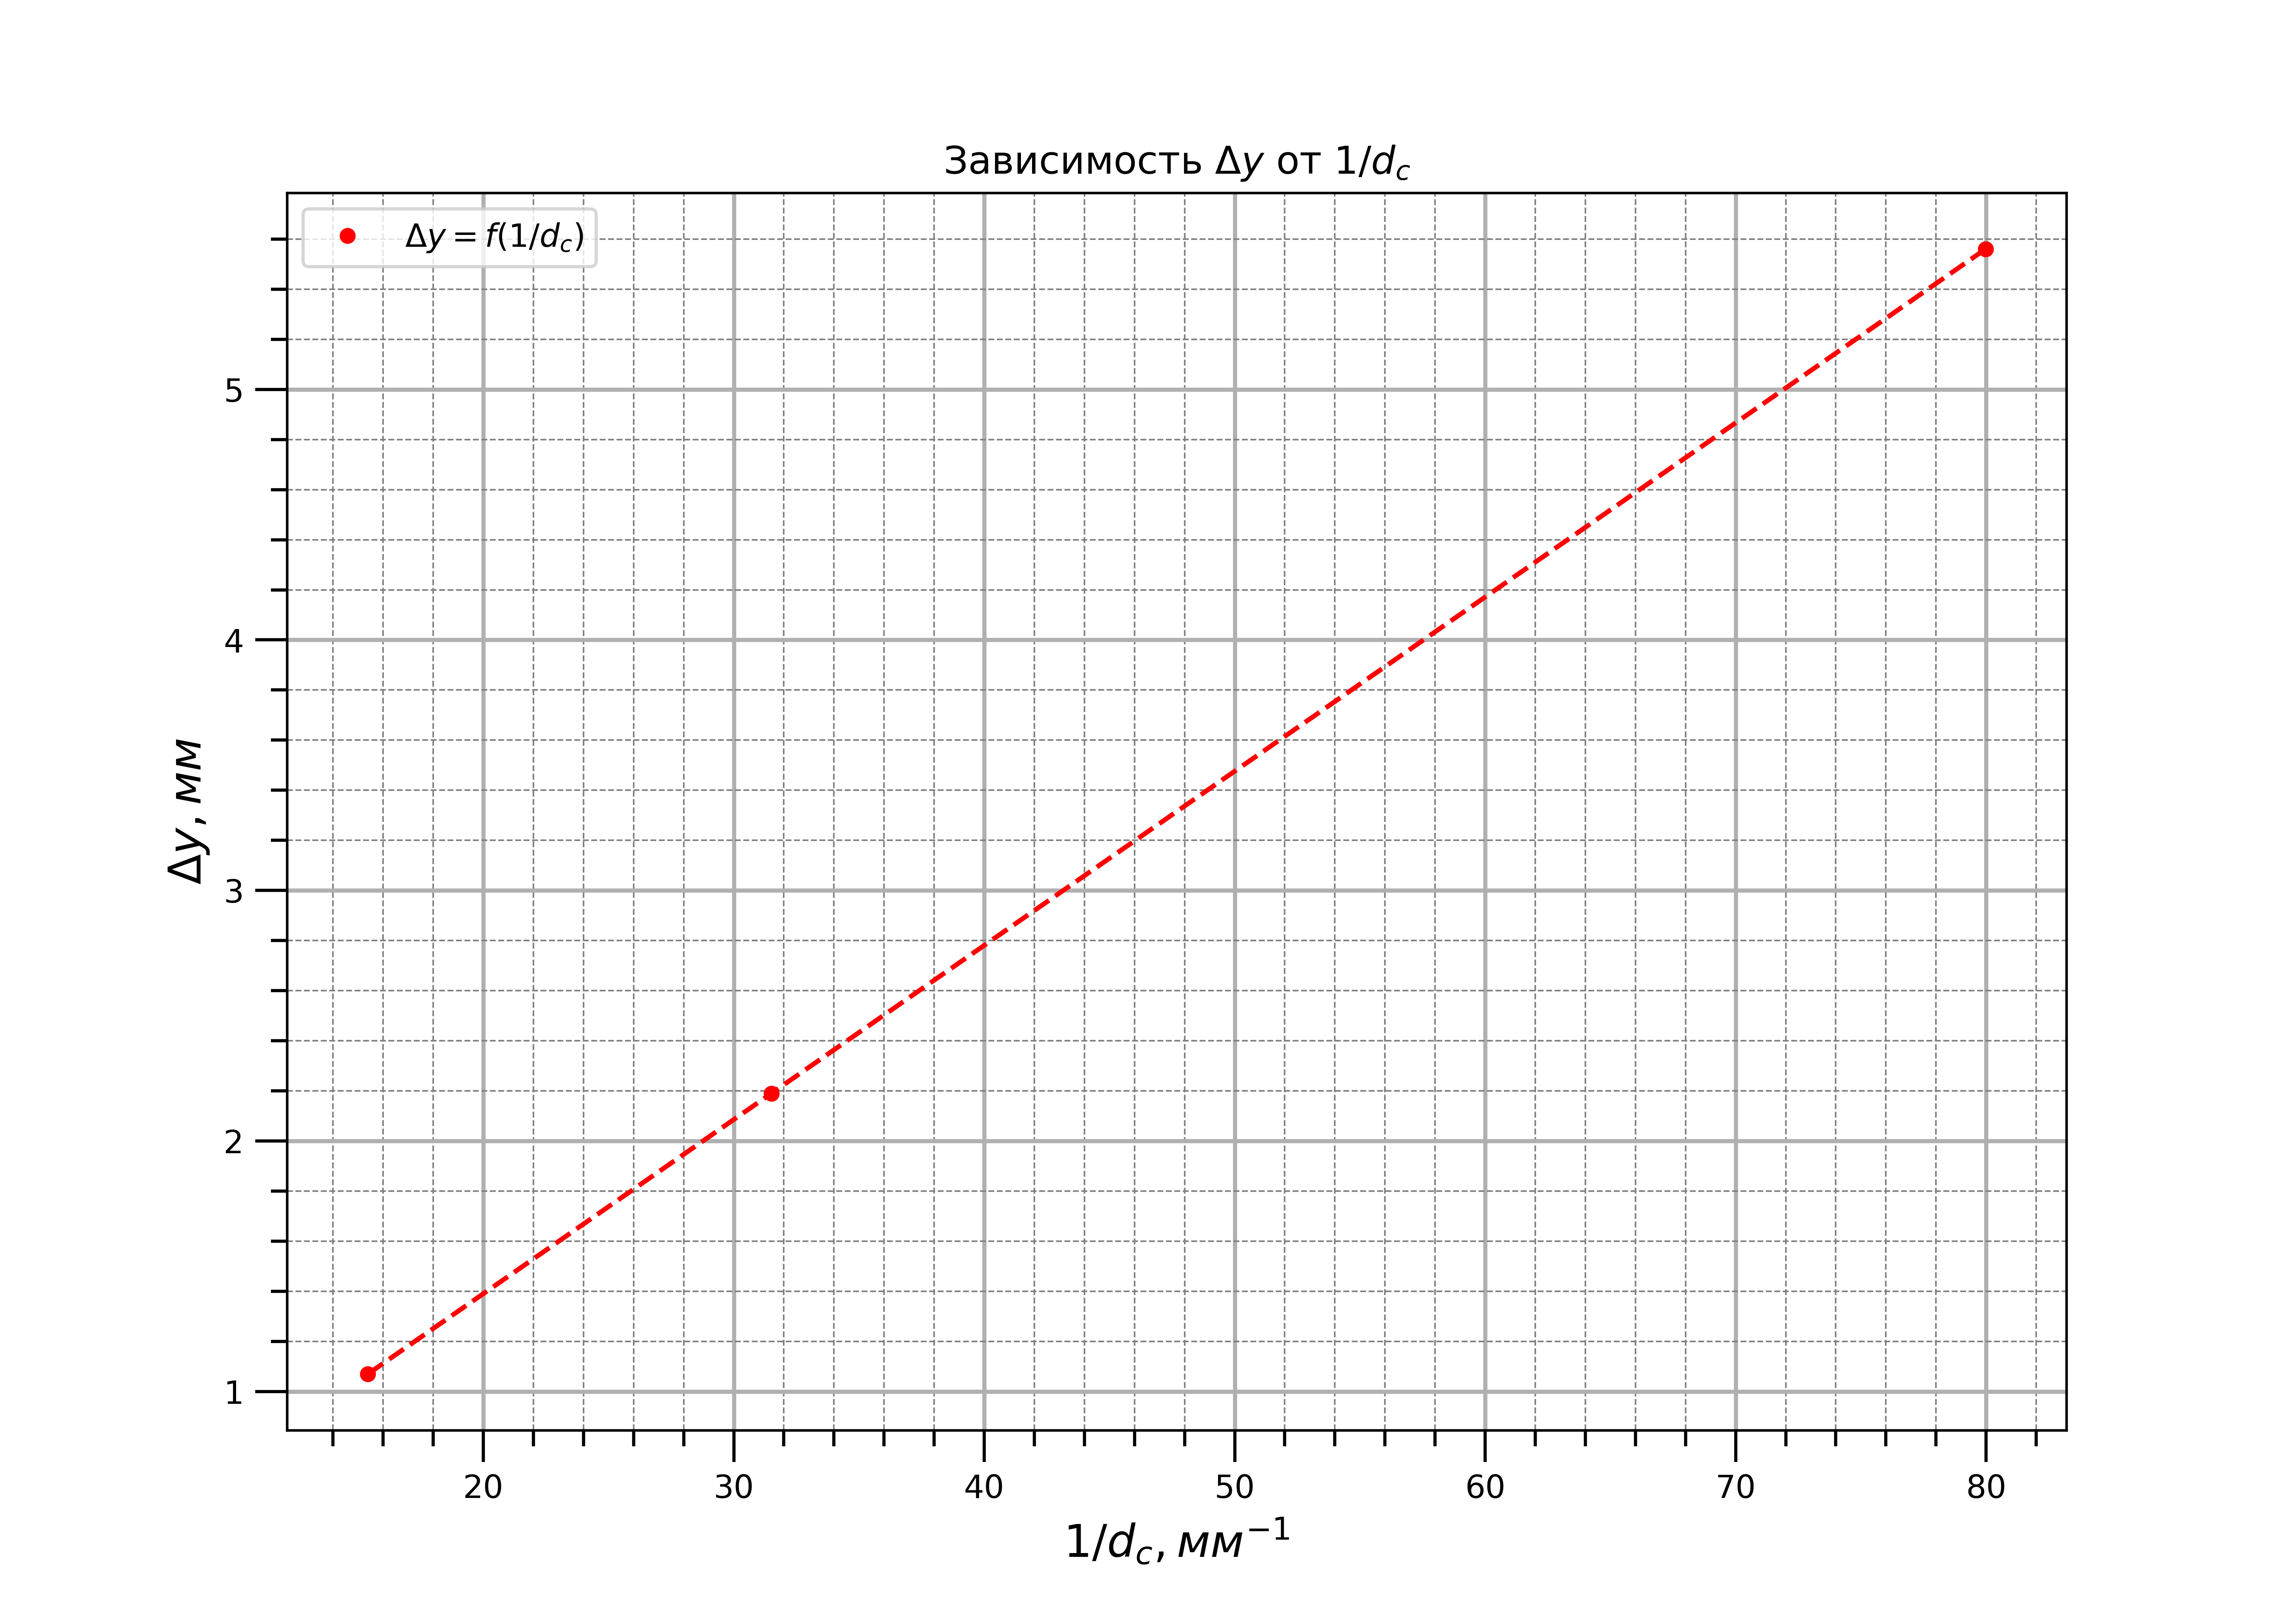
\includegraphics[width=0.6\linewidth]{dy.png}
			\caption{$\Delta y = f(1/ d_c)$}
		\end{center}
	\end{figure}
	
	
	
	

	
	
	
	\textbf{Обсуждение результатов и выводы: }\\
	
	
	В данной лабораторной работе мы исследовали преобразование Фурье в оптике, с помощью которого благодаря фурье-плоскости и фурье-образам рассчитали периоды сеток.
	
\end{document}
